% Options for packages loaded elsewhere
\PassOptionsToPackage{unicode}{hyperref}
\PassOptionsToPackage{hyphens}{url}
%
\documentclass[
  landscape]{article}
\usepackage{amsmath,amssymb}
\usepackage{lmodern}
\usepackage{iftex}
\ifPDFTeX
  \usepackage[T1]{fontenc}
  \usepackage[utf8]{inputenc}
  \usepackage{textcomp} % provide euro and other symbols
\else % if luatex or xetex
  \usepackage{unicode-math}
  \defaultfontfeatures{Scale=MatchLowercase}
  \defaultfontfeatures[\rmfamily]{Ligatures=TeX,Scale=1}
\fi
% Use upquote if available, for straight quotes in verbatim environments
\IfFileExists{upquote.sty}{\usepackage{upquote}}{}
\IfFileExists{microtype.sty}{% use microtype if available
  \usepackage[]{microtype}
  \UseMicrotypeSet[protrusion]{basicmath} % disable protrusion for tt fonts
}{}
\makeatletter
\@ifundefined{KOMAClassName}{% if non-KOMA class
  \IfFileExists{parskip.sty}{%
    \usepackage{parskip}
  }{% else
    \setlength{\parindent}{0pt}
    \setlength{\parskip}{6pt plus 2pt minus 1pt}}
}{% if KOMA class
  \KOMAoptions{parskip=half}}
\makeatother
\usepackage{xcolor}
\usepackage[left=1cm,right=1cm,top=1cm,bottom=1.5cm]{geometry}
\usepackage{graphicx}
\makeatletter
\def\maxwidth{\ifdim\Gin@nat@width>\linewidth\linewidth\else\Gin@nat@width\fi}
\def\maxheight{\ifdim\Gin@nat@height>\textheight\textheight\else\Gin@nat@height\fi}
\makeatother
% Scale images if necessary, so that they will not overflow the page
% margins by default, and it is still possible to overwrite the defaults
% using explicit options in \includegraphics[width, height, ...]{}
\setkeys{Gin}{width=\maxwidth,height=\maxheight,keepaspectratio}
% Set default figure placement to htbp
\makeatletter
\def\fps@figure{htbp}
\makeatother
\setlength{\emergencystretch}{3em} % prevent overfull lines
\providecommand{\tightlist}{%
  \setlength{\itemsep}{0pt}\setlength{\parskip}{0pt}}
\setcounter{secnumdepth}{-\maxdimen} % remove section numbering
\ifLuaTeX
\usepackage[bidi=basic]{babel}
\else
\usepackage[bidi=default]{babel}
\fi
\babelprovide[main,import]{ngerman}
% get rid of language-specific shorthands (see #6817):
\let\LanguageShortHands\languageshorthands
\def\languageshorthands#1{}


% Seitenzahlen unterdruecken:
\pagenumbering{gobble}


%Auf deutsche Captions einstellen:
\usepackage{caption}

\captionsetup{figurename=Abb., tablename=Tabelle}
%\usepackage[singlelinecheck=off]{caption}


% Spalten ermoeglichen:

\newenvironment{cols}[1][]{}{}

\newenvironment{col}[1]{\begin{minipage}{#1}\ignorespaces}{%
\end{minipage}
\ifhmode\unskip\fi
\aftergroup\useignorespacesandallpars}

\def\useignorespacesandallpars#1\ignorespaces\fi{%
#1\fi\ignorespacesandallpars}

\makeatletter
\def\ignorespacesandallpars{%
  \@ifnextchar\par
    {\expandafter\ignorespacesandallpars\@gobble}%
    {}%
}
\makeatother


\usepackage{float}
\ifLuaTeX
  \usepackage{selnolig}  % disable illegal ligatures
\fi
\IfFileExists{bookmark.sty}{\usepackage{bookmark}}{\usepackage{hyperref}}
\IfFileExists{xurl.sty}{\usepackage{xurl}}{} % add URL line breaks if available
\urlstyle{same} % disable monospaced font for URLs
\hypersetup{
  pdflang={de},
  hidelinks,
  pdfcreator={LaTeX via pandoc}}

\author{}
\date{\vspace{-2.5em}}

\begin{document}

\begin{cols}

\begin{col}{0.475\textwidth}
\includegraphics[width=4.85in,]{../../../../../../private/var/folders/qc/h0z4rw0d7gd2_9z6485zx5gw0000gp/T/Rtmp7Vp37w/file2f5618c92f3}

\begin{figure}[H]

{\centering 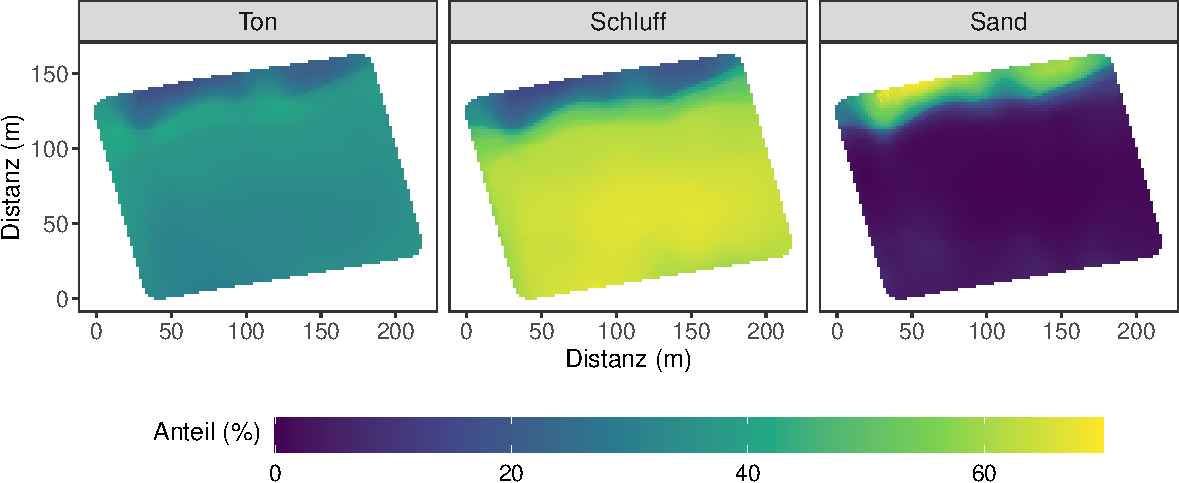
\includegraphics{S06_Fa_Voll_Feld_Altrheinwiesen_files/figure-latex/unnamed-chunk-8-1} 

}

\caption{Ton-, Schluff- und Sand-Anteil (\%) der Fläche Altrheinwiesen. Die räumliche Auflösung beträgt 2x2 Meter.}\label{fig:unnamed-chunk-8}
\end{figure}

\hfill\break

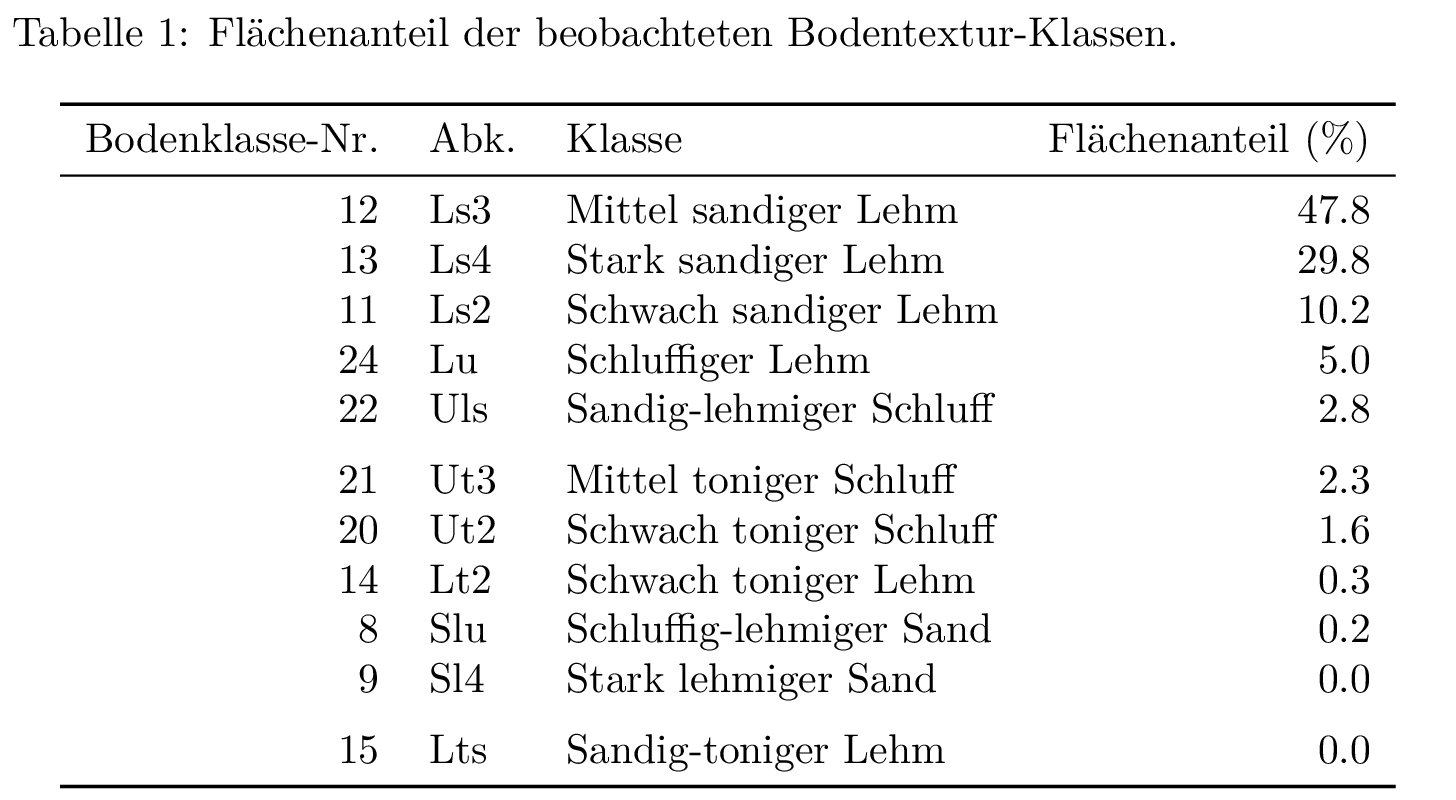
\includegraphics[width=1\linewidth,]{Tabelle1}

\end{col}

\begin{col}{0.05\textwidth}
.\\


\end{col}

\begin{col}{0.475\textwidth}

\begin{figure}[H]

{\centering 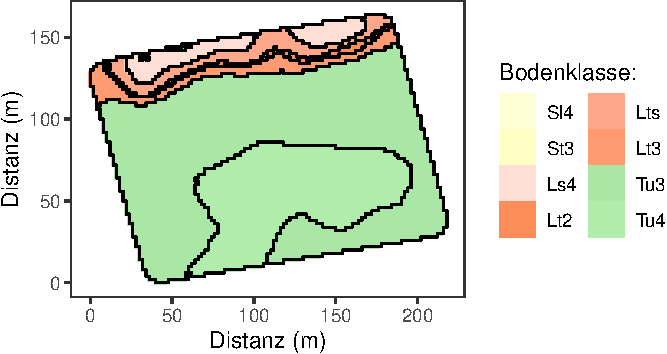
\includegraphics[width=0.6\linewidth,]{S06_Fa_Voll_Feld_Altrheinwiesen_files/figure-latex/unnamed-chunk-18-1} 

}

\caption{Karte der Bodentexturklassen auf der Grundlage des mit dem Geophilus gemessenen Ton-, Schluff- und Sandgehalts.}\label{fig:unnamed-chunk-18}
\end{figure}

\begin{figure}[H]

{\centering 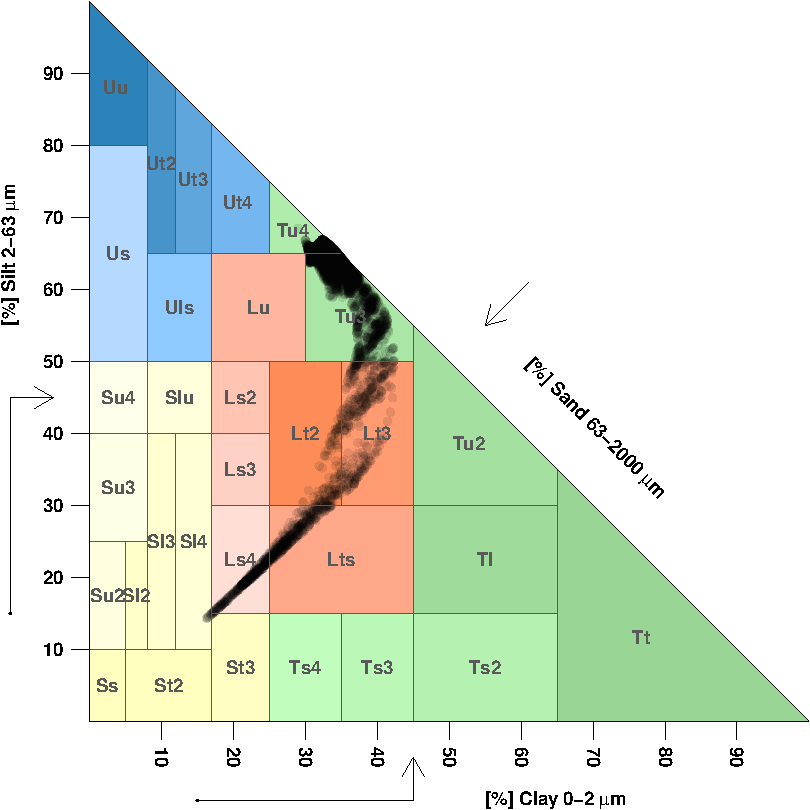
\includegraphics[width=0.6\linewidth,]{S06_Fa_Voll_Feld_Altrheinwiesen_files/figure-latex/unnamed-chunk-20-1} 

}

\caption{Bodentextur-Klasse der beobachteten Fläche. Aus den Karten extrahierte Klassen sind für jedes Pixel als Punkt markiert (schwarz). }\label{fig:unnamed-chunk-20}
\end{figure}

\end{col}

\end{cols}

\end{document}
